\vspace{-3mm}
\section{晶圆级 LLM 并行}\label{sec:meshmp}
\vspace{-1mm}

本节介绍晶圆级 LLM 并行方案，其中针对预填充、解码和 KV cache 管理都采用了新的设计。

\vspace{-3mm}
\subsection{预填充并行}
\vspace{-1mm}

LLM 预填充的并行方案必须符合 PLMR 模型。主要挑战包括：（i）预填充期间要处理多个大矩阵，因此需要有效划分维度以实现百万核心并行（P）；（ii）优化 GEMM 运算还涉及进一步划分，以及计算与通信的重叠，既要尽量降低长距离通信延迟（L），又要遵守本地内存约束（M）并考虑有限的路由资源（R）；（iii）连续 GEMM 运算经常需要矩阵转置，而转置在网格 NoC 上代价很高（L）。

\begin{figure}[t!]
    \centering
    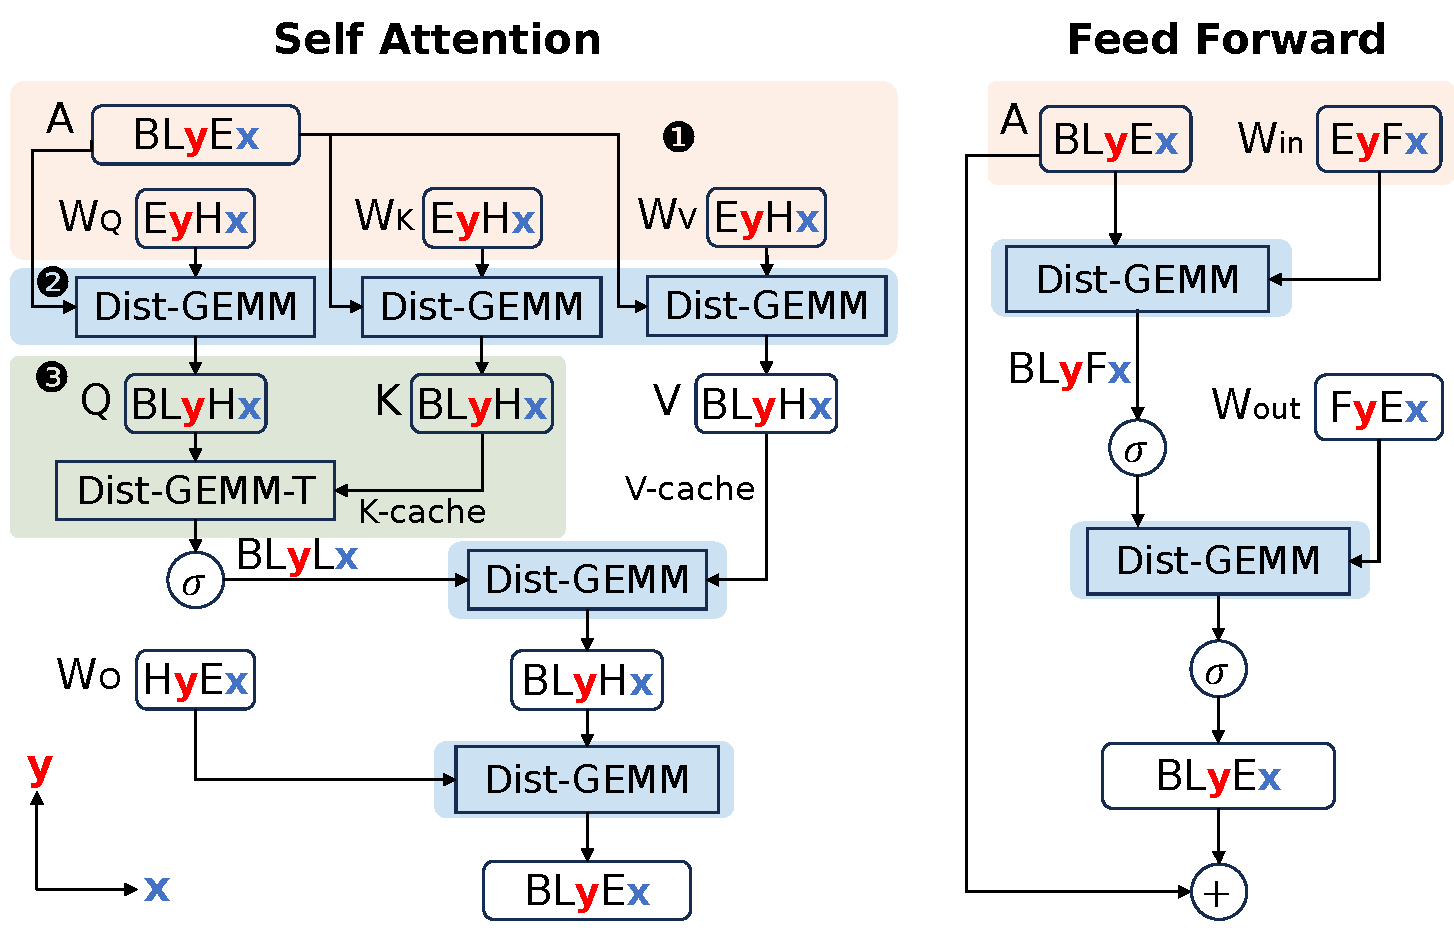
\includegraphics[width=0.46\textwidth]{imgs/prefill-partition.pdf}
    \vspace{-2mm}
    \caption{预填充并行方案。$E_xF_y$ 表示形状为 $EF$ 的矩阵，其中 $E$ 维沿网格核心的 $x$ 轴划分，$F$ 维沿 $y$ 轴划分。}
    \vspace{-5mm}
    \label{fig:prefill-partition}
\end{figure}

\mypar{为百万核心并行设计细粒度划分} 为获得较高芯片利用率，我们建议把输入激活矩阵和权重矩阵的两个维度同时沿核心的 $X$ 轴与 $Y$ 轴划分。与通常只划分嵌入维度的现有方法~\cite{flashattn2,flashdecoding++,megatron,google2023efficiently}相比，这种方法能够实现粒度更细的百万级并行；现有方法在 PLMR 设备上的并行度不足。

我们用自注意力和前馈模块说明这种划分，如图~\ref{fig:prefill-partition} 所示。为便于讨论，定义以下记号：预填充过程中，输入激活 $A$ 与权重 $W$ 都是多维张量。$B$ 表示 batch size，$L$ 表示序列维度\footnote{$L$：序列维度；L：PLMR 中的内存访问延迟。}，$E$ 表示嵌入维度，$H$ 表示注意力头维度，$F$ 表示前馈模块的隐藏维度。如图中的 \myc{1} 所示，$A$ 的划分布局记作 $BL_yE_x$，其中 $L$ 维沿核心的 $Y$ 轴划分，$E$ 维沿 $X$ 轴划分。所有权重矩阵（$W_Q$、$W_K$、$W_V$、$W_{in}$ 和 $W_{out}$）也同样沿两个维度划分。

\mypar{设计符合 PLMR 的分布式 GEMM}
如图~\ref{fig:prefill-partition} 中的 \myc{2} 所示，我们建议在预填充阶段，以新设计的、符合 PLMR 的分布式 GEMM 替代面向共享内存架构的传统 GEMM 算子。TPU 和 GPU 系统的 GEMM 主要依赖 allgather，而符合 PLMR 的分布式 GEMM 算法在遵守本地内存和路由约束的同时实现较高 NoC 带宽利用率，因而满足 L、M 和 R 属性。第~\ref{sec:gemm} 节将完整介绍该分布式 GEMM。

\mypar{使用转置式分布式 GEMM 避免矩阵转置}
我们为预填充提出一种免转置并行方案，以避免共享内存 LLM 系统中的常见操作——矩阵转置。PLMR 的 L 属性指出，矩阵转置在晶圆级设备上尤其昂贵：它可能要求网格一个角上的核心把数据发送到对角的另一角，从而形成长距离通信路径。

如图~\ref{fig:prefill-partition} 中的 \myc{3} 所示，我们的免转置并行方案使用转置式分布式 GEMM（记作 dist-GEMM-T）~\cite{summa,trans-dist}，计算 LLM 预填充中的 $Q@K^T$。具体而言，$Q$ 和 $K$ 中间张量分别由 $X$ 与 $W_Q$、$W_K$ 相乘得到；受片上划分形状影响，若采用普通 dist-GEMM，必须先转置 $K$，而 dist-GEMM-T 可以免去这一步。

\vspace{-3mm}
\subsection{解码并行}
\vspace{-1mm}

\begin{figure}[t!]
    \centering
    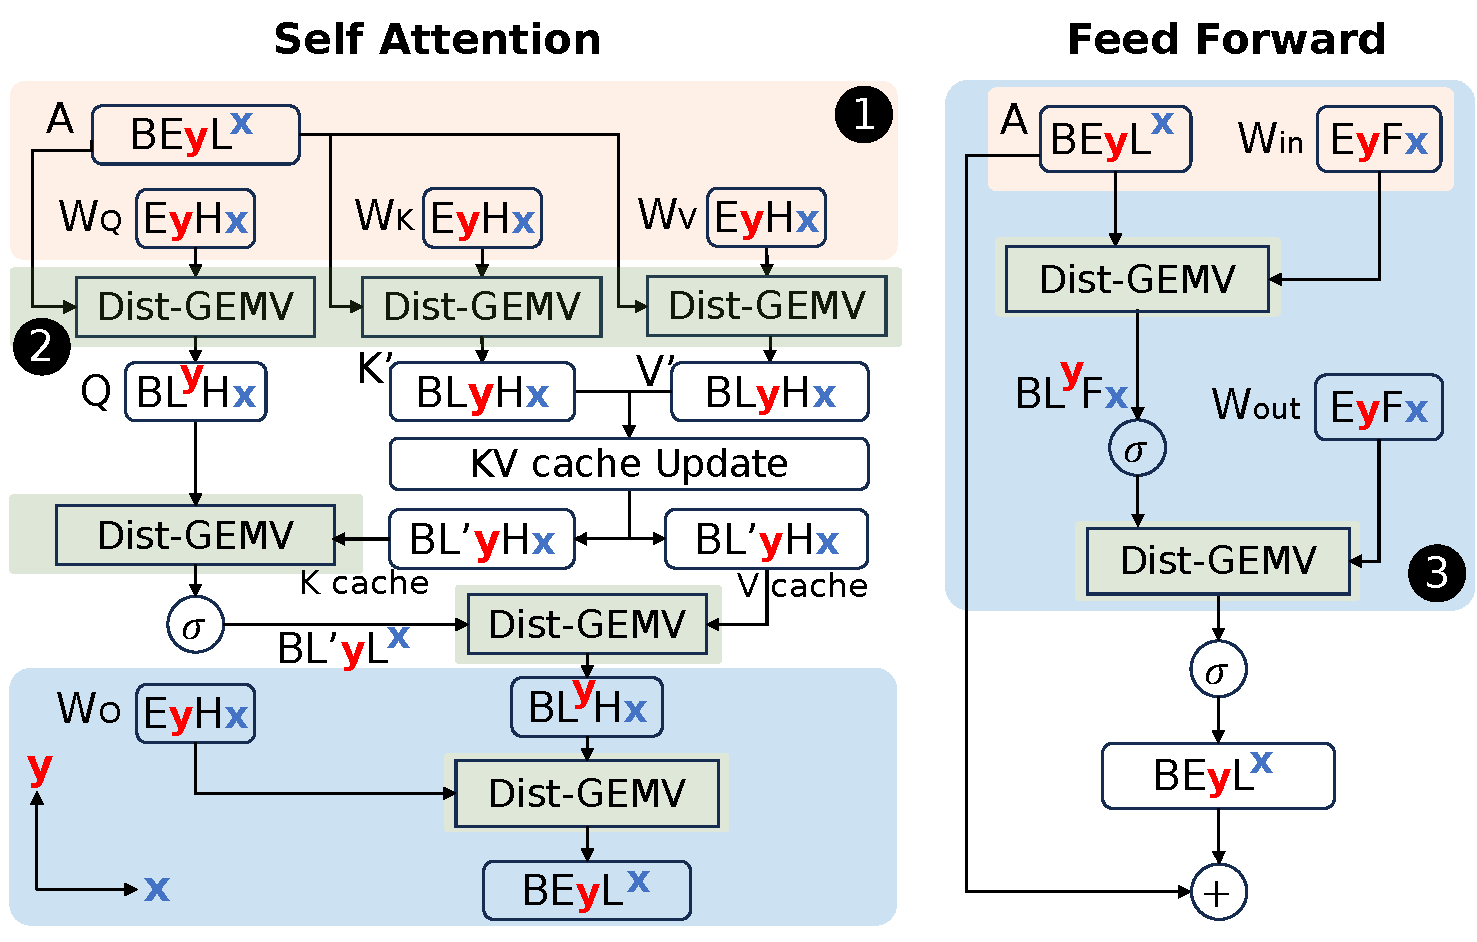
\includegraphics[width=0.46\textwidth]{imgs/decode-partition.pdf}
    \vspace{-2mm}
    \caption{解码并行方案。$E^yF_x$ 表示 $E$ 维沿 $y$ 轴复制，$F$ 维沿 $x$ 轴划分。}
    \vspace{-5mm}
    \label{fig:decode-partition}
\end{figure}

LLM 解码是内存带宽密集型阶段，其并行策略面临以下挑战：（i）受输入序列和 batch size 限制，解码使用的矩阵小于预填充，因此当维度不足以划分时必须谨慎并行；（ii）该阶段高度依赖 GEMV。GEMV 的计算强度低于 GEMM，计算阶段较短，难以充分与通信重叠，因此容易受到网格 NoC 长距离通信延迟（L）的影响，同时还要遵守本地内存和路由约束（M 和 R）；（iii）连续 GEMV 运算会引入 NoC 上代价高昂的矩阵转置，可能违反 L 属性。

\mypar{设计细粒度复制，以最低通信成本实现并行} 当张量维度不足以达到解码所需的高并行度时，我们建议对 LLM 张量进行细粒度复制，尤其是复制序列维度：预填充阶段的序列长度等于提示词长度，而解码阶段等于 1。这种方法有两项主要优势：（i）提高并行度，确保所有核心的负载均衡；（ii）避免跨全部核心的 allreduce 等额外通信。如图~\ref{fig:decode-partition} 中的 \circled{1} 所示，$E$ 维沿 $y$ 轴划分，$L$ 维沿 $x$ 轴复制，记作 $BE_yL^x$。权重矩阵 $W$ 仍沿两个维度划分，与预填充阶段一致。

我们的细粒度复制不同于近期的长上下文/序列推理系统~\cite{loongserve,distserve}；这些工作只在预填充而非解码阶段选择性地复制某些维度。

\mypar{设计符合 PLMR 的分布式 GEMV} 我们发现，现有 GEMV 实现因长距离通信和单核路由资源消耗过多而无法完整满足 PLMR。为此，我们提出符合 PLMR 的分布式 GEMV，并在整个解码阶段使用这一新实现，如图~\ref{fig:decode-partition} 中的 \myc{2} 所示。第~\ref{sec:gemv} 节将完整介绍其设计。

\mypar{预先优化模型权重放置以避免矩阵转置}
为避免解码期间的矩阵转置，我们针对解码，尤其是分布式 GEMV，预先优化模型权重布局。这样便可消除矩阵转置。尽管预填充与解码之间会产生重新放置的开销，但它远小于 token 生成期间连续执行矩阵转置的开销。

图~\ref{fig:decode-partition} 的 \myc{3} 展示了这一方案。具体来说，我们为解码时的分布式 GEMV 优化 $W_{O}$、$W_{out}$ 等权重的放置方式，使其不同于预填充阶段的布局。该方法还消除了在解码自注意力中计算 $Q@K^T$ 时的转置操作。

\vspace{-3mm}
\subsection{基于移位的 KV cache 管理}\label{sec:parallel:kvcache}
\vspace{-1mm}

\begin{figure}[t!]
    \centering
    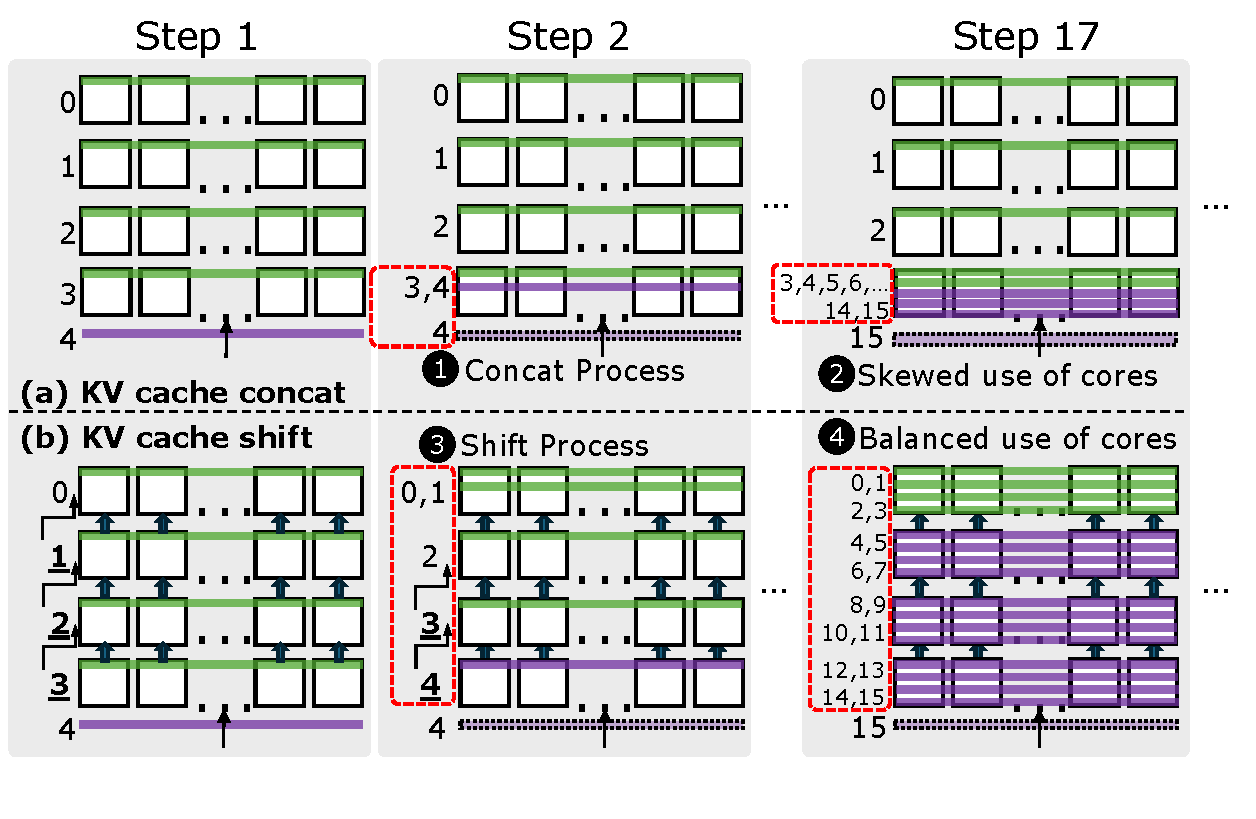
\includegraphics[width=1\linewidth]{imgs/KVManage.pdf}
    \vspace{-9mm}
    \caption{KV cache 拼接与 KV cache 移位的比较}
    \vspace{-5mm}
    \label{fig:kv_cache_update}
\end{figure}

在 PLMR 设备上管理 KV cache 很有挑战性：一方面，大量数据必须分布存储在多个核心上并遵守本地内存约束（M）；另一方面，KV cache 计算必须分散到多个核心以实现高并行度（P）。对此，我们得到以下认识。

\mypar{现有的拼接式管理造成核心利用率倾斜} 当前 KV cache 管理方法主要把最新生成的 KV 向量拼接到既有 cache 末尾。这一操作在共享内存架构上很高效，但在 PLMR 设备上会造成核心利用率严重倾斜。如图~\ref{fig:kv_cache_update} 的 \circled{1} 所示，每一行只有一个核心负责存储生成的 KV 向量并对其进行计算。生成若干 token 后，这个唯一的核心很快就会成为瓶颈，如图~\ref{fig:kv_cache_update} 的 \circled{2} 所示；这造成内存使用倾斜并违反 PLMR 中的 M。与此同时，KV cache 在核心间分布不均也会降低并行效率，违反 P 属性。

\mypar{提出基于移位的管理以均衡核心利用率} 我们提出基于移位的 KV cache 管理策略，把 cache 数据均匀分布到所有核心。该方法不把新的 KV cache 向量拼接到末尾，而是执行负载均衡移位：每一行把最旧的 KV cache 数据传给上一行，如图~\ref{fig:kv_cache_update} 的 \circled{3} 所示。新 KV 数据到达时，每个核心都会把本地容量与邻居进行比较；若容量相等，便触发向上移位，每一行从下一行接收数据，并把一部分数据传给上一行。如 \circled{4} 所示，这能保证 KV cache 均匀分布在所有核心上。

向上移位并行使用 NoC 链路，因此保持较高性能并满足 P 属性。KV cache 的物理放置与逻辑连续性一致，而且只在相邻核心之间移动数据，符合 L 属性。该方法还彻底解决了拼接式方案中最后一行核心违反 M 约束的问题。

\vspace{-3mm}
\subsection{实现细节}
\vspace{-1mm}

下面概述若干实现细节。

\mypar{预填充与解码的转换} 预填充和解码需要不同策略。为高效完成转换，我们通过高速 NoC 重新排列 KV cache 和权重。NoC 的聚合带宽通常达到数百 Pbit/s，因此可以即时完成，而无需依赖较慢的片外内存。

\mypar{并行配置} \sys 使用离线自动调优，为每个模型选择核心数量，并依据模型大小、输入/输出长度、单核内存以及预填充/解码阶段来优化延迟。系统会为两个阶段选择不同的核心数，而高带宽 NoC 支持快速动态重映射。对于输入/输出长度可变的模型，系统采用平均值以保持接近峰值的性能。每个模型都单独执行自动调优，以适配其具体需求。

\mypar{自注意力变体} \sys 支持分组查询注意力~\cite{gqa}、多头注意力~\cite{mha}和多查询注意力~\cite{mqa}等自注意力变体。它们先按注意力头维度分组，然后在组内执行 dist-GEMM、dist-GEMV 和 dist-GEMM-T。
